Um die partiellen Sudokus zu erstellen, auf Eindeutigkeit zu überprüfen und die Schwierigkeit zu bewerten,
werden immer wieder folgende Schritte durchlaufen:
\begin{enumerate}
    \item \label{step:fill} Markierte Felder mit Ziffern füllen
    \item \label{step:unique} Partielles Sudoku auf Eindeutigkeit überprüfen
    \item \label{step:permute} Permutation der Ziffern im partiellen Sudoku
    \item \label{step:difficulty} Bewertung des Schwierigkeitsgrads des partiellen Sudokus
\end{enumerate}
Im Lösungsmodus werden die Schritte~\ref{step:fill} und~\ref{step:permute} weggelassen.
Für die Modi, wo Felder markiert werden, auch wenn einzelne Ziffern gesetzt werden, werden alle Schritte durchlaufen.
Die genaue Ausführung der Schritte unterscheidet sich lediglich in Schritt~\ref{step:permute} und das der SAT-Solver zusätzliche Constraints erhält.
Wenn Schritt~\ref{step:unique} fehlschlägt, das heißt das Sudoku entweder nicht lösbar ist oder mehrere Lösungen hat,
wird Schritt~\ref{step:fill} wiederholt, bis ein valides partielles Sudoku gefunden wurde.

\subsection{Markierte Felder befüllen}
Zunächst befüllen wir die markierten Felder mit Ziffern.
Auch die Felder wo eine Ziffer gesetzt wurde, werden lediglich als markiert betrachtet.
Für die Befüllung der markierten Felder haben wir verschiedene Ansätze ausprobiert.

\subsubsection{Backtracking}
Der erste Ansatz war ein Backtracking-Algorithmus, der rekursiv versucht, die markierten Felder mit Ziffern zu füllen.
Wenn wir eine Belegung gefunden haben, die allerdings nicht lösbar oder mehrdeutig war, haben wir den Algorithmus weiterlaufen lassen,
bis eine eindeutige Lösung gefunden wurde, oder eine maximale Anzahl an Versuchen erreicht wurde.
Das Problem bei diesem Ansatz war, dass wir dadurch nur sehr ähnliche partielle Sudokus erhalten haben,
die wir überprüft haben.

\subsubsection{Zufälliges Backtracking}
Vom zufälligen Backtracking haben wir uns weniger Abhängigkeit der einzelnen partiellen Sudokus erhofft.
Im Prinzip haben wir normales Backtracking genutzt, mit dem Unterschied, dass wir die nächste Ziffer immer zufällig ausgewählt haben.
Wenn wir eine Belegung gefunden haben, die allerdings nicht lösbar oder mehrdeutig war,
haben wir den Algorithmus von vorne begonnen.
So gab es keine große Abhängigkeit zwischen den erzeugten partiellen Sudokus.
Das Problem bei diesem Ansatz und auch bei normalen Backtracking war,
dass fast alle partiellen Sudokus die wir überprüft haben, gar nicht lösbar waren.
Die Hinweise untereinander entsprachen zwar den Sudoku-Regeln, es war aber nicht möglich alle anderen Zellen korrekt mit Ziffern zu füllen.

\subsubsection{Grid auf Lösungen anwenden}
Als letzten Ansatz haben wir voll ausgefüllte Sudokus genommen und diese auf die markierten Felder angewendet.
Das heißt, an jeder markierten Zelle haben wir die Ziffer des voll ausgefüllten Sudokus dieser Zelle eingetragen.
Da wir die markierten Sudokus als Liste mit 81 Nullen und Einsen gespeichert haben,
ging dies durch zellenweise Multiplikation mit dem voll ausgefüllten Sudoku.
Dieser Ansatz hat sich als sehr effektiv herausgestellt, da so jedes partielle Sudoku mindestens eine Lösung hat.
Wir haben eine Datei mit 160.000 voll ausgefüllten Sudokus generiert, welche alle keine Unterquadrate enthalten.
Wie bereits in \cref{sec:unterquadrate} erwähnt ist es schwieriger eindeutige Lösungen zu finden, wenn Unterquadrate vorhanden sind.
Dafür haben wir das Programm von~\cite{stunmuffin_sudoku_generator_2025} modifiziert, dass nur vollständige Lösungen generiert werden
und diese danach auf Unterquadrate überprüft werden.

%TODO: Hier noch Pseudocode für die Anzahl Unterquadrate einfügen

\subsection{Überprüfung auf eindeutige Lösung}
\subsubsection{Vorüberlegungen}
Um zu überprüfen, ob bestimmte partielle Sudokus eindeutig lösbar sind, haben wir uns verschiedene Lösungsmöglichkeiten überlegt.
Die zwei wichtigsten Überlegungen waren ein CSP-Solver (Constraint Satisfaction Problem) oder ein SAT-Solver (Satisfiability).
Um herauszufinden, welcher dieser Ansätze eine schnellere Lösung bietet, haben wir ein Python-Skript geschrieben, welches diesen Sachverhalt untersuchen sollte~\cite{sat_csp_comparison}.

Dafür musste das Problem für die Löser umformuliert werden, einmal musste ein Sudoku also als Constraints und Dimensionen für den CSP-Solver formuliert werden.
Und zweitens muss man Sudoku auf SAT reduzieren.

\begin{enumerate}
    \item CSP-Solver \\
    Das Sudoku lässt sich elegant als CSP darstellen.
    Dafür betrachten wir das Spielfeld als Menge
    $$
    X = \{x_{i,j}|1 \leq i,j \leq n\}
    $$
    Jede Variable $x_{i,j}$ bekommt hier also eine Domäne von Werten, die gegeben ist durch $D(x_{i,j}) = \{1, 2, \dots, n$\}.
    Zuletzt müssen noch die Constraints angegeben werden.
    Für jede Zelle $z_{i, k}$ einer Reihe, dass $x_{i, k} \neq x_{j, k}$ mit $j \neq i$.
    Das Gleiche gilt für die Spalten, also $x_{i, k} \neq x_{i, l}$ mit $k \neq l$, und auch für die Untergitter.
    Die Hinweise eines Sudokus werden auch als Constraints gegeben.
    Wenn z.B. in der ersten Spalte und in der ersten Zeile eine 5 steht dann wäre die Variable $D(x_{1, 1}) = \{5\}$.

    %Um das Problem eines Sudokus in ein CSP zu übertragen haben wir schlicht die Domänen der Zellen auf die Werte $1, 2, \dots, 9$ gesetzt
    %und die Sudoku Regeln jeweils in Constraints übersetzt und anschließend die Domänen der schon vorgegebenen Zellen nur auf die eingegebenen Zahlen eingeschränkt.
    %Die Constraints waren also für jede Zelle $z_{i, k}$ einer Reihe, dass $z_{i, k} \neq z_{j, k}$ mit $j \neq i$.
    %Das Gleiche gilt für die Spalten, also $z_{i, k} \neq z_{i, l}$ mit $k \neq l$.
    %Für die Unterquadrate wurden jeweils auch wieder geprüft, dass jede Zelle nicht den gleichen Wert haben darf wie eine andere im Unterquadrat.

    \item SAT-Solver \\
    Um Sudokus auf SAT zu reduzieren müssen wir erst alle Variablen als Wahrheitswerte darstellen.
    Wir haben also eine Formel benutzt die jeder Kombination an Reihe,
    Spalte und jedem Wert einen einheitlichen Wahrheitswert zuweist.
    \begin{equation}
        V(r, c, d) = n^2 \cdot (r - 1) + n \cdot (c - 1) + d
    \end{equation}
    Weiter müssen wir jetzt das Sudoku als konjunktive Normalform darstellen.
    Als Erstes mussten wir festlegen, dass jede Zelle mindestens eine Zahl enthält, was mit dieser Menge an Klauseln dargestellt wurde:
    \begin{equation}
        \forall i, j, k: V(i, j, k) \text{ mit } i, j, k \in \{1, ..., n\} %TODO Werte und Reihen/Spalten gleiche Menge?
    \end{equation}
    und, dass jede Zelle maximal eine Zahl enthält, wiederum mit dieser Menge an Klauseln.
    \begin{equation}
        \forall i, j, k_1, k_2: \neg V(i, j, k_1) \vee \neg V(i, j, k_2) \text{ mit }i, j, k_1, k_2 \in \{1, ..., n\} \text{ und } k_1 \neq k_2
    \end{equation}
    Des Weiteren musste nun für jede Reihe, jede Spalte und jedes Untergitter bestimmt werden, dass zwei Zellen nicht den gleichen Wert und alle Werte $1, \dots, n$
    in der Zeile, Spalte oder dem Untergitter enthalten sein müssen.
    Das funktioniert gleich wie bei den Regeln für das ganze Sudoku nur das die $i, j$ Werte entweder auf die Reihe, die Spalte oder das Untergitter beschränkt ist.
    Wir ver-unden also anschließend alle Klauseln, die wir erstellt haben, dadurch kann der SAT-Solver sie lösen.
    Um die Hinweise hinzuzufügen, nimmt man also an, dass bestimmt Variablen wahr sind und löst dann mit dieser Annahme das SAT-Problem.
\end{enumerate}

Um die Lösungsansätze miteinander vergleichen zu können, haben wir jeweils 100 4x4, 6x6 und 9x9 Sudokus lösen lassen.
Hierfür haben wir einmal den cadical SAT-Solver~\cite{pysat} verwendet und außerdem die verschiedenen Solver einer CSP-Solver library~\cite{pycsp}.
Wir haben einmal den Durchschnitt der Zeiten pro Solver für das reine Lösen ausgewertet und die Anzahl der abgelaufenen Durchläufe, also die Durchläufe die über eine Sekunde gedauert haben.
Die Ergebnisse lassen sich \cref{fig:sat_csp_comparison} entnehmen.

\begin{figure*}[h!]
    \centering

    \begin{subfigure}[b]{0.8\textwidth}
        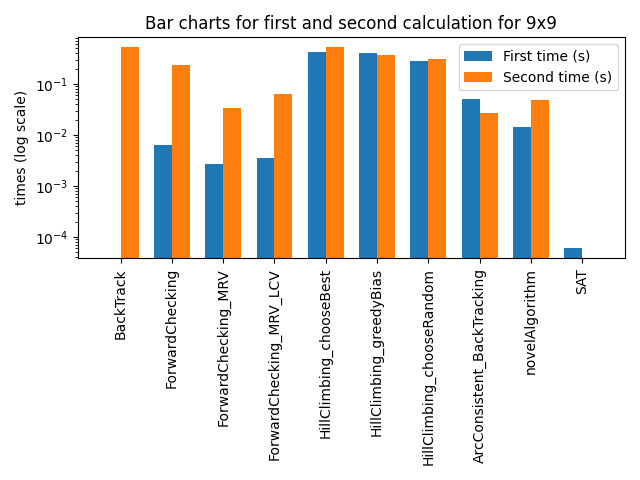
\includegraphics[width=\textwidth]{Pictures/times_9x9}
        \caption{times 9x9}
    \end{subfigure}
    \hfill
    \begin{subfigure}[b]{0.8\textwidth}
        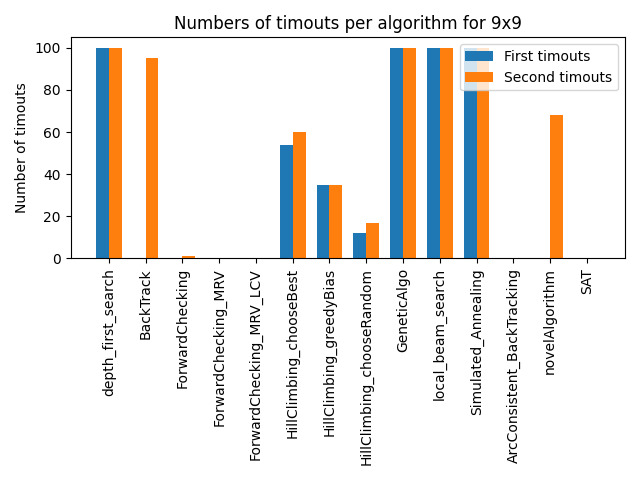
\includegraphics[width=\linewidth]{Pictures/timeouts_9x9}
        \caption{timeouts 9x9}
    \end{subfigure}

    \caption{Comparison of times and timeouts for different solving Algorithms}
    \label{fig:sat_csp_comparison}
\end{figure*}

Wie man unschwer erkennen kann, ist der SAT-Solver mit Abstand am schnellsten und löst die Sudokus innerhalb von meist nicht messbarer Zeit.
Genau gleich sieht es mit den Timeouts aus, bei allen 100 Sudokus hat der SAT-Solver Lösungen gefunden.
Viele der anderen Solver haben keine einzige Lösung in der gegebenen Zeit gefunden.
Auch wenn manche CSP-Lösungsverfahren gut abgeschnitten haben, macht es keinen Sinn etwas anderes als den getesteten SAT-Solver zu verwenden.
Wir können mit ähnlicher Performanz rechnen, da auch cadical-rs so wie die Implementierung in Python auf ersichtlich schnellem Code in C/C++ laufen.

\subsubsection{vorgegebene Ziffern}
Wenn einige Ziffern vorgegeben sind, müssen wir dem SAT-Solver zusätzliche Constraints geben.
Uns interessieren dabei nicht die genauen Werte der Ziffern sondern ihre Beziehung untereinander.
Für zwei Zellen $z_{i, j}$ und $z_{x, y}$ in denen die gleiche Ziffer vorgegeben ist, müssen wir folgende Klauseln hinzufügen:
\begin{equation}
    \forall k: (\neg V(i, j, k) \lor V(x,y, k)) \land  (V(x, y, k) \lor \neg V(k, l, k)) \text{ mit }k \in \{1, ..., n\}
\end{equation}
Das ist gleich zur Äquivalenz von den Werten der Zelle.

Für zwei Zellen $z_{i, j}$ und $z_{k, l}$ in denen unterschiedliche Ziffern vorgegeben sind, müssen wir folgende Klauseln hinzufügen:
\begin{equation}
    \forall k: \neg V(i, j, k) \lor \neg V(x, y, k) \text{ mit }k \in \{1, ..., n\}
\end{equation}
Sie sorgen dafür, dass in den Zellen nicht die gleiche Ziffer steht.

\subsubsection{Implementierung}
Um zu überprüfen ob ein Sudoku eindeutig ist, nutzen wir \cref{alg:eindeutig}.
Wenn durch die Anwendung des Grids auf die Lösungen ein eindeutig lösbares Sudoku entsteht, können wir dieses dem Nutzer zurückgeben.
In ~\cref{alg:generierung} wird dargestellt, wie wir dabei vorgehen.

\begin{algorithm}
    \caption{Sudoku eindeutig lösbar}
    \label{alg:eindeutig}
    \begin{algorithmic}[1]
        \Require $G$ ist ein leeres oder teilweise ausgefülltes $9 \times 9$ Sudoku-Gitter.
        \Require $Solver$ ist eine SAT-Solver mit den entsprechenden Sudoku Klauseln.
        \Ensure Es wird \textbf{true} und die Lösung zurück gegeben wenn das Sudoku eindeutig lösbar ist und \textbf{false} wenn nicht.
        \Function{Eindeutig}{$G, Solver$}
            \State Let $solvable, solution \gets \Call{Solver.solveSudoku}{G}$
            \If{solvable}
                \State $\Call{Solver.prohibitSolution}{solution}$
                \State Let $unique, uniqueSolution \gets \Call{Solver.solveSudoku}{G}$
                \State \Return (unique, $uniqueSolution$)
            \Else
                \State \Return \textbf{false}
            \EndIf
        \EndFunction
    \end{algorithmic}
\end{algorithm}


\begin{algorithm}
    \caption{Sudoku Generierung}
    \label{alg:generierung}
    \begin{algorithmic}[1]
        \Require $G$ ist ein Sudoku-Gitter mit Einsen an markierten und Nullen and unmarkierten Stellen.
        \Require $M$ Menge an vollständigen Sudokus, die wir zur Generierung nutzen.
        \Function{generateSudoku}{$G, M$}
            \State Let $solver \gets \Call{Solver}{G.size}$
            \For{$m \in M$}
                \State Let $transformed \gets G \cdot m$ \Comment{Stellenweise Multiplikation}
                \State Let $unique, solution \gets \Call{Eindeutig}{transformed, solver}$
                \If{$unique$}
                    \State \Return $solution$
                \EndIf
            \EndFor

        \EndFunction
    \end{algorithmic}
\end{algorithm}

Beim Generieren wurden zwei verschiedene Möglichkeiten verglichen, einmal die Generierung ohne und einmal mit Threads.
Das Generieren zu parallelisieren scheint sinnvoll, da es keine großen Abhängigkeiten voneinander gibt.
Die Implementierung mit Threads ist im Grunde die gleiche wie ohne, nur, dass hier die Menge $M$ in die Anzahl von Threads viele disjunktive Teilmengen geteilt wird.
Anschließend wird auf jeder Thread auf einer dieser Teilmengen gestartet. Sobald eine Lösung gefunden wird, werden die anderen Threads unterbrochen.

\subsection{Permutation der Zahlen}
Da alle Lösungsdateien in der ersten Zeile 1 bis 9 geordnet stehen haben, müssen wir die Ziffern in den partiellen Sudokus permutieren.
Beim normalen Markierungsmodus wird die Permutation der Ziffern zufällig gewählt.
Beim Markierungsmodus mit Eingabe von wenigen Ziffern wird die Permutation so gewählt, dass an den markierten Zellen mit Ziffern,
dort auch diese Ziffern stehen.
Durch die zusätzlichen Constraints ist dies immer möglich.


\subsection{Schwierigkeit bewerten}


\subsection{Evaluation}
Um die Qualität des Backends zu bestimmen, haben wir unseren Algorithmus auf 100.000 Sudokus angewendet.
Dazu haben wir das Datenset aus \cite{tdoku_data_zip} verwendet und haben dort wo eine Zahl steht einen allgemeinen Hinweis gesetzt.
Dadurch haben wir Sudokus mit 21 bis 31 Hinweisen erhalten, für die es jeweils eindeutig lösbare partielle Sudokus gibt.
Für diese haben wir anschließend den Algorithmus auf dem Nekton-Server laufen lassen.
Die Ergebnisse wie oft ein Sudoku gefunden wurde sind in \cref{tab:ergebnisse} abgebildet.

\begin{table}[H]
    \centering
    \begin{tabular}{|c|c|c|c|}
        \hline
        \textbf{Anzahl Hinweise} & \textbf{Anzahl true} & \textbf{Anzahl total} & \textbf{Wahrscheinlichkeit} \\
        \hline
        21 & 0     & 3     & 0.00\% \\
        22 & 4     & 147   & 2.72\% \\
        23 & 786   & 1829  & 42.97\% \\
        24 & 10883 & 11879 & 91.62\% \\
        25 & 30508 & 30638 & 99.58\% \\
        26 & 33783 & 33786 & 99.99\% \\
        27 & 16948 & 16948 & 100.00\% \\
        28 & 4235  & 4235  & 100.00\% \\
        29 & 513   & 513   & 100.00\% \\
        30 & 21    & 21    & 100.00\% \\
        31 & 1     & 1     & 100.00\% \\
        \hline
    \end{tabular}
    \caption{Übersicht: Anzahl Hinweise, Anzahl true, Anzahl total und Wahrscheinlichkeit (in Prozent) pro Wert}
    \label{tab:ergebnisse}
\end{table}

Die Zeit, die zum Finden einer Belegung gebraucht wurde, ist mit den blauen Balken in \cref{fig:zeiten} dargestellt.
Mit den orangenen Balken ist die Zeit dargestellt, die das Backend gerechnet hat, bevor die Suche aufgegeben wurde.

\begin{figure}[H]
    \centering
    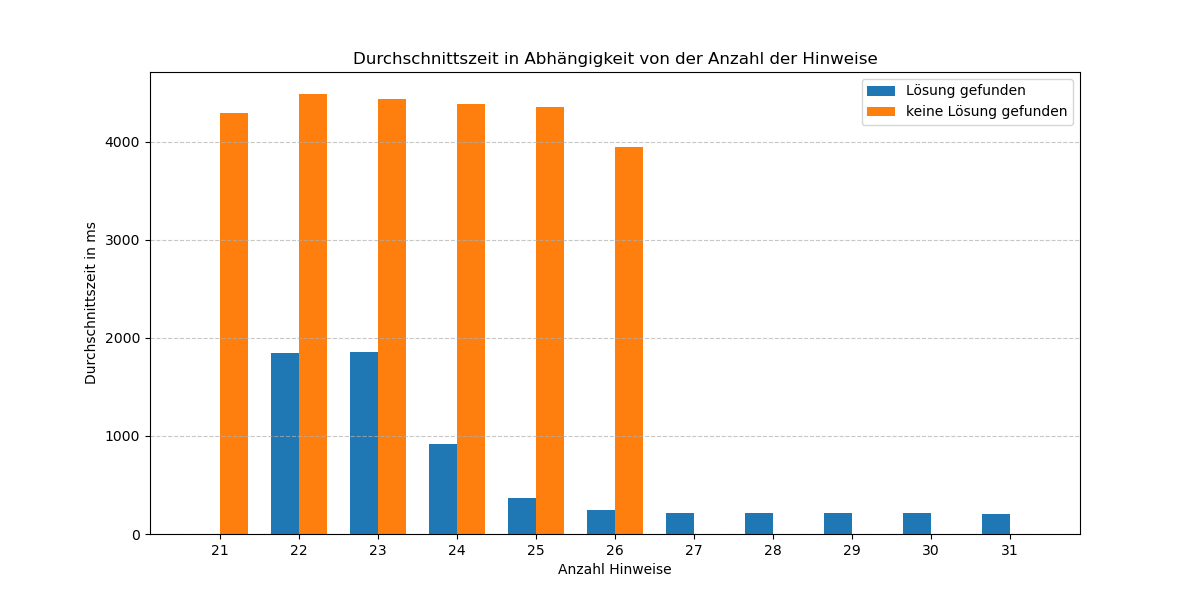
\includegraphics[width=0.8\textwidth]{Pictures/zeiten}
    \caption{Zeiten die für die Berechnung benötigt wurden}
    \label{fig:zeiten}
\end{figure}

Man sieht, dass der Algorithmus für Sudokus mit 24 oder mehr Hinweisen fast immer eine Belegung findet und dafür im Schnitt deutlich kürzer als eine Sekunde braucht.
Bei zufälligen Lösungen, ohne Einschränkung an die Unterquadrate wurden Sudokus mit 24 Hinweisen nur in unter 60\% der Fälle gefunden.
Sudokus mit weniger als 24 Hinweisen wurden gar nicht gefunden in unseren Tests.
Das heißt, die Generierung von Lösungen mit keinen Unterquadraten hat die Qualität des Backends deutlich verbessert.

\subsection{Experiment mit CUDA}

Aufgrund der stark parallelen Natur des Problems haben wir ebenfalls einen GPU-basierten Ansatz mithilfe von CUDA untersucht. Dabei wurden sowohl ein CSP- als auch ein SAT-Ansatz implementiert und getestet.
Für Sudokus mit vielen vorgegebenen Hinweisen erzielte die GPU-Lösung vergleichbare Ergebnisse zum CPU-basierten Lösen (Hardware: Nvidia RTX 1050ti vs. AMD Ryzen 7 2700X). Bei Sudokus mit wenigen Vorgaben hingegen schnitt der GPU-Ansatz schlechter ab als die CPU-Lösung.

Dies führen wir insbesondere auf das komplexe \emph{Branching} zurück, welches sich nur bedingt für GPUs eignet. Aufgrund des höheren Aufwands und der geringeren Effizienz haben wir uns letztlich trotz des interessanten Experiments für den CPU-basierten Ansatz entschieden, da dieser einfacher und performanter ist.